\documentclass[a4paper,titlepage]{article}
\usepackage[parfill]{parskip}
\usepackage[utf8x]{inputenc}
\usepackage[english]{babel}
\usepackage[T1]{fontenc}
\usepackage{graphicx}
\usepackage{float}
\usepackage[final]{pdfpages}
\usepackage{listings}
\usepackage[colorlinks=true, allcolors=blue]{hyperref}
\usepackage[a4paper,top=3cm,bottom=2cm,left=3cm,right=3cm,marginparwidth=1.75cm]{geometry}

% lstset for setting styles for source code
\lstset{ %
  backgroundcolor=\color{white},   % choose the background color; you must add \usepackage{color} or \usepackage{xcolor}; should come as last argument
  basicstyle=\footnotesize,        % the size of the fonts that are used for the code
  breakatwhitespace=true,         % sets if automatic breaks should only happen at whitespace
  breaklines=true,                 % sets automatic line breaking
  captionpos=b,                    % sets the caption-position to bottom
  commentstyle=\color{blue},    % comment style
  extendedchars=true,              % lets you use non-ASCII characters; for 8-bits encodings only, does not work with UTF-8
  keepspaces=true,                 % keeps spaces in text, useful for keeping indentation of code (possibly needs columns=flexible)
  identifierstyle=\color{purple},
  keywordstyle=\color{orange},       % keyword style
  language=Verilog,                 % the language of the code
  morekeywords={*,char,int,struct,bool},           % if you want to add more keywords to the set
  rulecolor=\color{black},         % if not set, the frame-color may be changed on line-breaks within not-black text (e.g. comments (green here))
  showspaces=false,                % show spaces everywhere adding particular underscores; it overrides 'showstringspaces'
  showstringspaces=false,          % underline spaces within strings only
  showtabs=false,                  % show tabs within strings adding particular underscores
  stepnumber=2,                    % the step between two line-numbers. If it's 1, each line will be numbered
  stringstyle=\color{red},     % string literal style
  tabsize=2,	                   % sets default tabsize to 2 spaces
  title=\lstname                   % show the filename of files included with \lstinputlisting; also try caption instead of title
}


\graphicspath{ {images/} }

\begin{document}

\begin{titlepage}
\vspace*{\fill}

\newcommand{\HRule}{\rule{\linewidth}{0.5mm}} % Defines a new command for the horizontal lines, change thickness here

\center % Center everything on the page

%----------------------------------------------------------------------------------------
%TITLE SECTION
%----------------------------------------------------------------------------------------

{ \huge \bfseries IoT Security Project}\\[0.4cm] % Title of your document

%----------------------------------------------------------------------------------------
%HEADING SECTIONS
%----------------------------------------------------------------------------------------

\textsc{\LARGE Sean Caster, Vincenzo Piscitello, Ryan Howerton, Terri Hewitt, and Adam Barton}\\[0.5cm] % Name of your university/college
\textsc{\Large Senior Design}\\[0.5cm] % Major heading such as course name
\textsc{\large Fall 2018}\\[2.5cm] % Minor heading such as course title


%\HRule \\[0.8cm]
\begin{minipage}{.8\textwidth}  % Set width of abstract
%\HRule \\[0.8cm]
\textbf{\large Abstract} \\
\HRule \\[0.4cm]
Write an abstract here. Lorem ipsum dolor sit amet, consectetur adipiscing elit, sed do eiusmod tempor incididunt ut labore et dolore mana aliqua. Ut enim ad minim veniam, quis nostrud exercitation ullamco laboris nisi ut aliquip ex ea commodo consequat. Duis aute irure dolor in reprehenderit in voluptate velit esse cillum dolore eu fugiat nulla pariatur. Excepteur sint occaecat cupidatat non proident, sunt in culpa qui officia deserunt mollit anim id est laborum
\\[0.4cm]
\HRule \\[1.5cm]
\end{minipage}
%\HRule \\[1.5cm]

                %----------------------------------------------------------------------------------------
                %DATE SECTION
                %-----------------    -----------------------------------------------------------------------

{\large \today}\\[3cm] % Date, change the \today to a set date if you want to be precise

%----------------------------------------------------------------------------------------
%LOGO SECTION
%------   ----------------------------------------------------------------------------------

%
\includegraphics{Logo}\\[1cm] % Include a department/university logo - this will require the graphicx package

%----------------------------------------------------------------------------------------

\vfill % Fill the rest of the page with whitespace

\end{titlepage}

\tableofcontents
\newpage

\section{Introduction}


\begin{figure}[H]
\centering
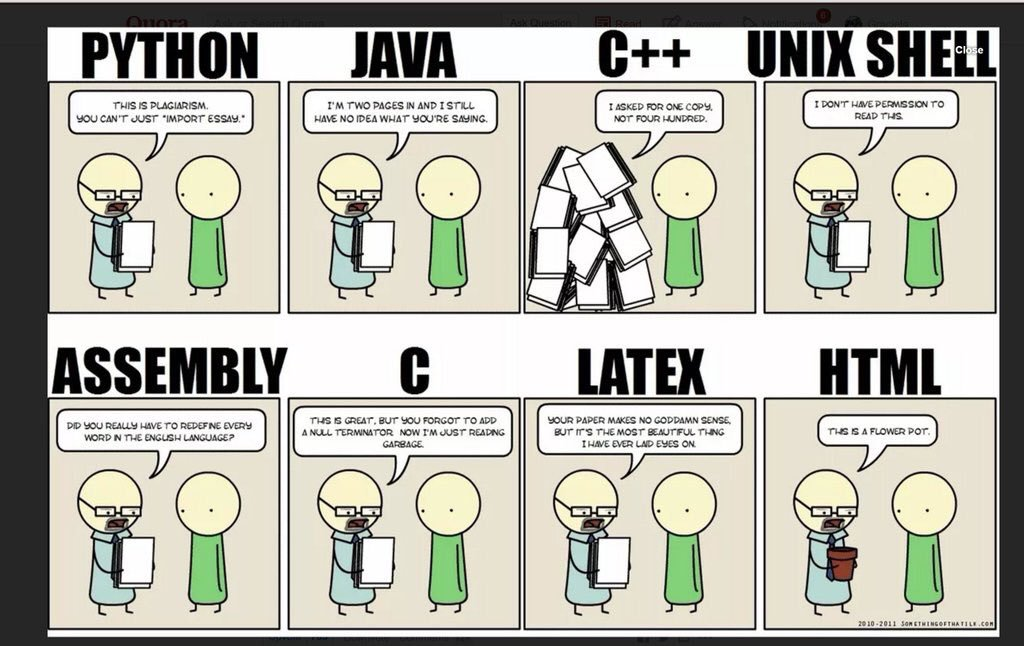
\includegraphics[width=15cm]{Images/coding-jokes.jpg}
\caption{Insert caption here. \href{https://www.google.com/}{© Google, 2017.}}
\end{figure}

Lorem ipsum dolor sit amet, consectetur adipiscing elit, sed do eiusmod tempor incididunt ut labore et dolore magna aliqua. Ut enim ad minim veniam, quis nostrud exercitation ullamco laboris nisi ut aliquip ex ea commodo consequat. Duis aute irure dolor in reprehenderit in voluptate velit esse cillum dolore eu fugiat nulla pariatur. Excepteur sint occaecat cupidatat non proident, sunt in culpa qui officia deserunt mollit anim id est laborum \cite{Example1}.

\subsection{Subsection}

Lorem ipsum dolor sit amet, consectetur adipiscing elit, sed do eiusmod tempor incididunt ut labore et dolore magna aliqua. Ut enim ad minim veniam, quis nostrud exercitation ullamco laboris nisi ut aliquip ex ea commodo consequat. Duis aute irure dolor in reprehenderit in voluptate velit esse cillum dolore eu fugiat nulla pariatur \cite{Example2}. Excepteur sint occaecat cupidatat non proident, sunt in culpa qui officia deserunt mollit anim id est laborum.

{\em Example Table:}

\begin{center}
\begin{tabular}{ c c c c c c}
 1 & 2 & 3 & 4 & 5 & 6\\ 
 7 & 8 & 9 & 10\\  
 11 & 12 & 13 & 14\\

\end{tabular}
\end{center}


\subsubsection{Subsubsection}

Lorem ipsum dolor sit amet, consectetur adipiscing elit, sed do eiusmod tempor incididunt ut labore et dolore magna aliqua. Ut enim ad minim veniam, quis nostrud exercitation ullamco laboris nisi ut aliquip ex ea commodo consequat. Duis aute irure dolor in reprehenderit in voluptate velit esse cillum dolore eu fugiat nulla pariatur. Excepteur sint occaecat cupidatat non proident, sunt in culpa qui officia deserunt mollit anim id est laborum.

\pagebreak

\section{Appendix}

\subsection{Design Synthesis and Analysis}

Lorem ipsum dolor sit amet, consectetur adipiscing elit, sed do eiusmod tempor incididunt ut labore et dolore magna aliqua. Ut enim ad minim veniam, quis nostrud exercitation ullamco laboris nisi ut aliquip ex ea commodo consequat. Duis aute irure dolor in reprehenderit in voluptate velit esse cillum dolore eu fugiat nulla pariatur. Excepteur sint occaecat cupidatat non proident, sunt in culpa qui officia deserunt mollit anim id est laborum.

Lorem ipsum dolor sit amet, consectetur adipiscing elit, sed do eiusmod tempor incididunt ut labore et dolore magna aliqua. Ut enim ad minim veniam, quis nostrud exercitation ullamco laboris nisi ut aliquip ex ea commodo consequat. Duis aute irure dolor in reprehenderit in voluptate velit esse cillum dolore eu fugiat nulla pariatur. Excepteur sint occaecat cupidatat non proident, sunt in culpa qui officia deserunt mollit anim id est laborum.

\subsection{Source Code}

\subsubsection{top\_module}
\lstinputlisting{./source/top_module.sv}

\subsection{Subsection}

\textbf{Source code listing}
\begin{lstlisting}
    vsim.work.n64_send_cmd
    add wave *
    force clk_1M 0 0, 1 {1ns} -r 2 ns
    force output_enable 1 @ 0
    force read_start 0 @ 0
    run 100 ns
\end{lstlisting}

\pagebreak

\bibliographystyle{ieeetr}
\bibliography{citations}

\end{document}
